\documentclass[letterpaper,twocolumn,10pt]{article}
\usepackage[hidelinks]{hyperref}
\usepackage{usenix2019_v3}
\usepackage{amsmath,amssymb,amsthm}
\newtheorem{theorem}{Theorem}
\usepackage{booktabs}
\usepackage{graphicx}
\usepackage{xspace}
\usepackage{tikz}
\usetikzlibrary{arrows.meta,positioning,calc}
\usepackage[capitalise,noabbrev]{cleveref}

\newcommand{\sys}{Barry\xspace}

\begin{document}

% CFP: short papers carry the prefix in the submitted title; it is not published.
\title{\Large \bf Short Paper: \sys: A Streaming Storage Engine for Temporal Graphs}

% Double-blind: no author identification.
\author{Anonymous submission}

\maketitle

\begin{abstract}
Temporal graphs whose edges are immutable timestamped events---audit
streams, agent execution traces, interaction logs---are ingested as
never-ending, near-sorted streams; queried along time and causality;
and retained under time-based policies. No deployed storage layer
serves this combination: entity-keyed graph stores demote the
timestamp to a payload attribute, columnar and LSM engines pay a join
per traversal hop, versioned temporal graph stores assume few
property-rich versions per entity, and statically time-sorted layouts
answer queries well while being unable to ingest at all.

\sys keys storage on time itself: each timestamp maps to a virtual
address by a constant-time shift, and demand paging absorbs temporal
sparsity, so no index is built or maintained. Ingestion becomes a
lock-free $O(1)$ append independent of arrival order; retention
becomes a page release over an address prefix; compaction is explicit
and off the ingest path; queries remain correct \emph{during}
concurrent ingestion through a per-slot publication protocol; and
because engine state is a pure function of the edge multiset, recovery
is re-ingestion. We evaluate \sys against a columnar engine, three CSR
layouts, and the most recent versioned temporal graph store, with
element-wise answer verification, on fourteen datasets including a
billion-edge enterprise corpus, and show that keying storage on time
wins the streaming and traversal axes by orders of magnitude while
conceding bounded, measured costs on the structural axis.
\end{abstract}

% =====================================================================
\section{Introduction}
\label{sec:intro}

A growing class of graphs is built from \emph{events}: a system call
touches a file, an agent invokes a tool, a host authenticates to
another, a user replies to a message. Each edge carries the moment it
happened, never changes afterwards, and arrives as part of a stream
that does not end. The queries such graphs exist to answer are
temporal and causal: \emph{what could have influenced this state},
\emph{what did this event go on to touch}, \emph{what did the
neighborhood look like at time $t$}, \emph{how much happened in this
window}. And because the value of an event fades with age, the data is
governed by time-based retention.

Every mature storage engine approaches this workload with a layout
built for something else. Dynamic graph stores---packed-memory-array,
tree, and adjacency-list designs~\cite{wheatman2021ppcsr, shen2026dcsr,
dhulipala2019aspen, fuchs2023sortledton}---key storage on source-vertex
identity and treat the timestamp as payload, so any time-constrained
query degrades to a structural scan with per-edge filtering, and any
retention pass must find expired edges wherever vertex order scattered
them. Columnar and LSM engines~\cite{raasveldt2019duckdb} invert the
failure: ordered by time, they answer range filters well, but every
hop of a traversal becomes a fresh join against the edge table.
Versioned temporal graph databases~\cite{li2026tva, hou2024aeong}
solve a genuinely different problem---retrieving the valid
\emph{version} of an updated entity---and their machinery presumes few,
property-rich versions per entity, an assumption an event stream
violates by design. Finally, a statically time-sorted CSR answers
temporal queries near-optimally and is not a storage engine at all:
its only update path is a rebuild, during which it is blind.

\sys starts from an address-space observation: a 64-bit virtual
address space is orders of magnitude larger than the time range of any
recorded workload. Rather than maintaining an index from timestamp to
location, \sys makes the timestamp \emph{be} the location:
\begin{equation}
A(T) \;=\; A_{\mathrm{base}} + \big((T - T_{\mathrm{start}}) \gg S\big)\times P,
\label{eq:mapping}
\end{equation}
a subtraction and a shift, with the operating system's demand paging
absorbing sparsity at zero data-structure cost. The properties the
workload needs then fall out of the layout rather than being
engineered on top of it. Because an edge's home is computed, not
searched, ingestion is a wait-free slot claim; because the computation
ignores arrival order, out-of-order and late events cost nothing;
because retention is a monotone time predicate, expiry is a release of
an address prefix; and because nothing is ever updated in place,
crash recovery collapses to replaying an append-only log through the
normal insert path.

This design has costs, and a storage paper owes their measurement as
much as their mitigation. A layout that refuses to organize by entity
must pay something on entity-keyed operations; a layout that never
sorts on ingest must either scan unsorted neighborhoods or compact
them later. We quantify both, delimit them with an explicit
compaction contract---\emph{always appendable, always correct,
including mid-ingest; fast neighborhood expansion after a compaction
schedulable at leisure}---and show the concessions are bounded
constants while the wins are orders of magnitude
(\cref{sec:eval}).

We contribute: (i)~a storage design that keys temporal graphs on time,
with formal guarantees for its addressing, space, granularity
selection, concurrency, and recovery (\cref{sec:design}); (ii)~a
concurrent-correctness protocol under which readers never observe a
torn or unpublished edge during lock-free multi-writer ingestion;
and (iii)~an evaluation methodology that verifies element-wise answer
equality across engines before reporting any latency, decomposes
algorithm time into storage-read share, and measures what a static
structure silently loses while rebuilding (\cref{sec:eval}).

% =====================================================================
\section{Design}
\label{sec:design}

\begin{figure}[t]
\centering
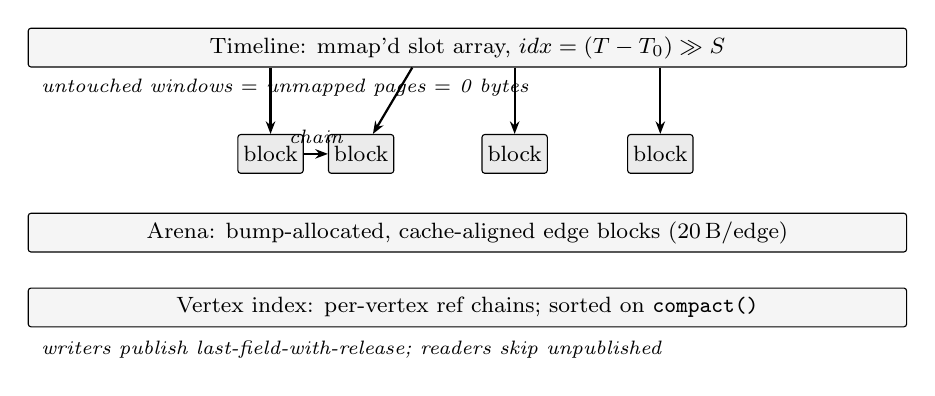
\begin{tikzpicture}[
  font=\footnotesize,
  box/.style={draw, rounded corners=1pt, minimum height=1.4em, inner sep=2pt},
  lbl/.style={font=\scriptsize\itshape},
  arr/.style={-{Stealth[length=1.6mm]}, thick}
]
\node[box, minimum width=0.92\columnwidth, fill=black!4] (tl) at (0,0)
  {Timeline: mmap'd slot array, $idx = (T - T_0) \gg S$};
\node[lbl, anchor=north west] at ($(tl.south west)+(0.05,-0.02)$)
  {untouched windows $=$ unmapped pages $=$ 0 bytes};
\node[box, fill=black!8] (b1) at (-2.5,-1.35) {block};
\node[box, fill=black!8] (b2) at (-1.35,-1.35) {block};
\node[box, fill=black!8] (b3) at (0.6,-1.35) {block};
\node[box, fill=black!8] (b4) at (2.45,-1.35) {block};
\draw[arr] ($(tl.south)+(-2.5,0)$) -- (b1);
\draw[arr] ($(tl.south)+(-0.7,0)$) -- (b2);
\draw[arr] ($(tl.south)+(0.6,0)$) -- (b3);
\draw[arr] ($(tl.south)+(2.45,0)$) -- (b4);
\draw[arr] (b1) -- (b2) node[midway, above, lbl] {chain};
\node[box, minimum width=0.92\columnwidth, fill=black!4] (ar) at (0,-2.35)
  {Arena: bump-allocated, cache-aligned edge blocks (20\,B/edge)};
\node[box, minimum width=0.92\columnwidth, fill=black!4] (vi) at (0,-3.3)
  {Vertex index: per-vertex ref chains; sorted on \texttt{compact()}};
\node[lbl, anchor=north west] at ($(vi.south west)+(0.05,-0.05)$)
  {writers publish last-field-with-release; readers skip unpublished};
\end{tikzpicture}
\caption{\sys's layout. The timestamp computes the timeline slot;
blocks hold the window's edges in arrival order; the vertex index adds
entity-keyed access and is the only structure compaction ever sorts.}
\label{fig:arch}
\end{figure}

\subsection{Time-keyed addressing}
\Cref{eq:mapping} maps a timestamp to a slot in a single anonymous
memory mapping (\cref{fig:arch}). Two properties make this an engine
rather than a trick.

\begin{theorem}[Addressing]
\label{thm:addr}
For any timestamp $t$, the slot holding every edge stamped $t$ is
computed in $O(1)$ worst case, with no data-dependent memory access.
\end{theorem}

\begin{theorem}[Space]
\label{thm:space}
With page size $P$ and $W_{occ}$ non-empty windows, resident timeline
memory is at most $W_{occ}\cdot P$ plus lazily materialized page-table
overhead; untouched windows cost zero bytes.
\end{theorem}

Sparsity is absorbed by the MMU, not by a structure the engine
maintains. The mapping is \emph{anonymous}---no file backing---so the
documented failure modes of file-backed mmap buffer
management~\cite{crotty2022mmap} (torn file pages, SIGBUS on
truncation, eviction stalls) do not arise; \sys uses mmap the way an
allocator reserves address space, not as a buffer pool. The shift $S$
is chosen adaptively from stream statistics; the selected window
occupancy is provably within $[\mathrm{target}/2,\,
4\cdot\mathrm{target})$, the factor-of-two slack on each side being
the honest price of power-of-two addressing. Proofs of all theorems
appear in the anonymized supplemental report.

\subsection{Lock-free ingestion, correct concurrent reads}
\label{sec:design-ingest}
An insert computes its slot (\cref{thm:addr}), claims an index in the
window's current block by a single \texttt{fetch\_add}, and installs
overflow blocks by CAS; every CAS failure implies another insert
succeeded, so ingestion is lock-free with wait-free slot claims.
Nothing sorts, nothing rebalances, and arrival order is
irrelevant---the property that separates \sys from every
sorted-on-ingest design the moment events straggle.

Concurrent readers are protected by a publication protocol rather
than locks. A writer fills an edge's payload first and stores its
timestamp \emph{last} with release semantics; since fresh arena pages
are zero-filled, a zero timestamp identifies an unpublished slot, and
readers acquire-load and skip it. Vertex-index refs publish through
their block pointer identically. One ordering rule makes the
optimized read path sound as well: an append clears the bucket's
\emph{sorted} flag \emph{before} bumping its counter, so any reader
that still observes the flag after an acquiring counter-read is
provably looking at a fully compacted, fully published prefix, and
may binary-search it.

\begin{theorem}[Concurrent reads]
\label{thm:conc}
Under the publication protocol, no query observes a torn, partial, or
unpublished edge during concurrent multi-writer ingestion, and every
query result equals that of some serially consistent state.
\end{theorem}

\subsection{The compaction contract}
Appends leave a vertex's neighborhood in arrival order, so a
time-windowed expansion costs $O(d)$. An explicit
\texttt{compact()} pass sorts each neighborhood by timestamp once,
after which expansion binary-searches in $O(\log d + k)$. Compaction
is deliberately \emph{not} on the insert path: folding it in would
make every batch pay for the whole index and forfeit streaming.
Queries are correct in either state---compaction changes cost, never
answers. The resulting contract is the paper's central trade: a
statically sorted structure gets its speed by making sorting
\emph{mandatory} and paying with a blind rebuild window
(\cref{sec:eval-stream}); \sys makes sorting \emph{optional} and pays
a bounded constant until it runs.

\subsection{Retention and durability}
Retention is a monotone time predicate, so under \cref{eq:mapping} it
is an address-prefix operation: \texttt{evict\_before($t$)} walks the
timeline prefix, merges block extents, and returns whole pages with
\texttt{madvise}; readers of other windows are undisturbed. For
durability, \sys exploits a property databases rarely enjoy: engine
state is a pure function of the edge multiset. The write-ahead log is
therefore just framed, checksummed batches of raw edges, an
asynchronous writer overlaps it with insertion, and recovery is
replaying the log through the normal insert path---no undo, no redo,
no idempotence bookkeeping; a torn tail frame is detected and
discarded.

% =====================================================================
\section{Implementation}
\label{sec:impl}
\sys is $\sim$6,300 lines of dependency-free C++17: the engine, nine
graph algorithms including bidirectional time-respecting traversal,
converters for two audit-log formats, and seven correctness suites
(among them a multi-writer/multi-reader stress test of
\cref{thm:conc} and an end-to-end synthetic-provenance fixture).
Interior windows of a range scan are copied without any timestamp
comparison---only boundary windows can contain out-of-range
edges---and boundary scans are AVX2-vectorized over the packed
edges. Source, converters, proofs, and every experiment driver will
be released.

% =====================================================================
\section{Evaluation}
\label{sec:eval}

\textbf{Setup.} 20-core Xeon, 188\,GB RAM, Ubuntu 20.04. Fourteen
datasets: LANL enterprise authentication (1.05B events, 17,666 hosts,
58 days)~\cite{lanl2015data}, DARPA TC whole-system provenance
(CADETS 22.5M and THEIA 97.3M information-flow edges over 2.9M/6.9M
entities), and 12 SNAP temporal graphs (60K--646M edges). Baselines:
DuckDB v1.5.5 through its C API in the same process; a time-sorted
CSR (\texttt{tcsr}, the strongest static competitor); an
arrival-order entity CSR (\texttt{ucsr}, what an ingesting
entity-keyed store holds between rebuilds); the topology-only CSR;
and TVA~\cite{li2026tva}, the most recent PVLDB temporal graph store,
via its released artifact. Every cross-engine latency in this section
is preceded by element-wise answer verification. Latency
distributions on this workload are heavy-tailed; we report medians
with tails or size-binned results, never means.

\subsection{Ingestion}
\label{sec:eval-ingest}
\begin{figure}[t]
\centering
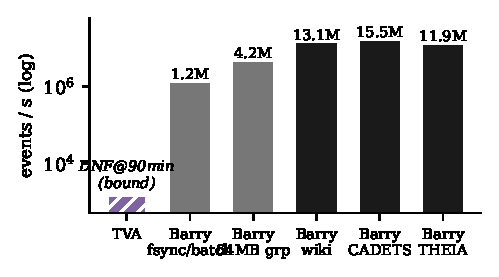
\includegraphics[width=\columnwidth]{figures/fig_ingest.pdf}
\caption{Single-thread ingestion (log scale). TVA is a bound: it did
not finish wiki-talk's 7.8M events within a 90-minute cutoff at
41.6\,GB RSS. \sys's durable modes pay the disk, not the engine.}
\label{fig:ingest}
\end{figure}
\begin{table}[t]
\centering\small
\caption{Cross-engine operations, identical data and thread count.
Snapshot = full-graph as-of scan. TVA row is a bound (DNF at the
90-minute cutoff); a sorted CSR has no ingest path to measure.}
\label{tab:e15}
\begin{tabular}{@{}llrrrr@{}}
\toprule
Engine & Dataset & Ingest & Pt.\ scan & Snapshot & RSS \\
\midrule
\sys & wiki-talk & 0.60\,s & 0.2\,$\mu$s & 0.65\,s & 0.7\,GB \\
\sys & CADETS    & 1.45\,s & 0.1\,$\mu$s & 218\,s  & 1.8\,GB \\
\sys & THEIA     & 8.16\,s & 0.4\,$\mu$s & 45.8\,s & 7.7\,GB \\
TVA  & wiki-talk & $>$5,415\,s & --- & --- & $>$41.6\,GB \\
\bottomrule
\end{tabular}
\end{table}
\sys ingests at 11.9--15.5M events/s single-threaded across
wiki-talk, CADETS, and THEIA (\cref{tab:e15}), and sustains 6.8M events/s on the
billion-edge LANL corpus under 12 concurrent writers \emph{while} 4
readers issue validated queries (48,636 queries, 780M edges checked,
zero protocol violations, final count exact). With the write-ahead
log enabled, durable ingestion reaches 4.2M events/s under 64\,MB
group commit against 7.4M volatile---bounded by the disk's measured
156\,MB/s sequential bandwidth, not by the engine---and 1.2M with an
fsync per batch. Driving TVA's artifact with the same single-threaded
event stream did not complete wiki-talk within a 90-minute cutoff at
41.6\,GB RSS (\cref{fig:ingest}): under event streams, every repeated
$(src,dst)$ contact extends one edge's version chain, the structure
its hopscotch layout must keep within bounded offsets, and its
design assumption---few, property-rich versions per entity---inverts.
A statically sorted CSR is absent from this comparison for the
simplest reason: it has no ingest path at all.

\subsection{Time-respecting traversal}
\label{sec:eval-traversal}
\begin{figure}[t]
\centering
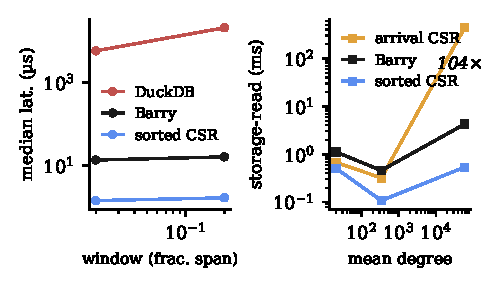
\includegraphics[width=\columnwidth]{figures/fig_traversal.pdf}
\caption{Left: traversal-to-fixpoint median latency vs.\ query window
(sx-mathoverflow); answers verified identical. Right: time-windowed
BFS storage-read time vs.\ mean degree; at provenance-scale degrees
the arrival-order entity store must scan what \sys's compacted
buckets skip.}
\label{fig:traversal}
\end{figure}
On multi-hop time-respecting traversal run to fixpoint, \sys leads
DuckDB by $150$--$700\times$ across all answer sizes---at
$|R|>1{,}000$ the median is 12\,ms against 2.43\,s---because each hop
costs a relational engine a join against the edge table
(\cref{fig:traversal}, left). The time-sorted CSR remains
$2.7\times$ faster than \sys at high degree: that is the measured
price of refusing to sort on ingest, and \cref{sec:eval-stream}
prices what the CSR pays for the privilege. Against the
\emph{ingesting} entity-keyed layout the ordering flips with degree
(\cref{fig:traversal}, right): at mean degree 20 \texttt{ucsr} wins
on contiguity, at 337 \sys reaches parity, and at LANL's mean degree
of 59,517 \sys leads by $104\times$ (4.2\,ms vs.\ 435\,ms)---the
crossover lands where event-stream workloads actually live. On
time-\emph{range} filtering, DuckDB's home ground, \sys's vectorized
scan wins the median $10.6\times$ (77\,$\mu$s vs.\ 819\,$\mu$s,
five seeds) with p95 at parity (981 vs.\ 1{,}105\,$\mu$s,
overlapping ranges). Decomposing classic graph algorithms (BFS,
PageRank, label propagation) into storage-read share under identical,
checksum-verified executions bounds the structural concession:
\sys delivers adjacency within $1.4$--$2.1\times$ of the topology-only
CSR optimum---at billion-edge scale, $1.4\times$---while being the
only layout of the four that ingests. \sys's weakest operation is the
full-graph as-of snapshot (enumerate-then-reduce; 218\,s on CADETS,
whose hottest vertices carry millions of events): precisely the
operation TVA's version-skipping is built to serve, and we report it
as its win.

\subsection{Rebuild versus stream}
\label{sec:eval-stream}
\begin{figure}[t]
\centering
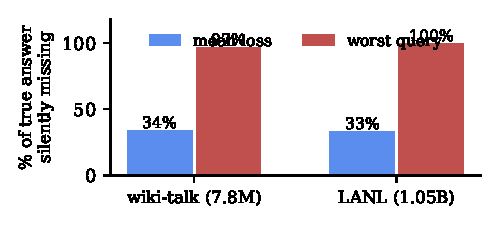
\includegraphics[width=\columnwidth]{figures/fig_rebuild.pdf}
\caption{What queries lose when served by a statically sorted
structure during its rebuild window, measured against the
always-current answer.}
\label{fig:rebuild}
\end{figure}
The time-sorted CSR's only update path is a full rebuild (28.4\,s on
LANL). Queries about the live window served from the pre-rebuild
snapshot are not stale but silently \emph{wrong}: on LANL, 68 of 100
queries returned incomplete answers, losing 33.2\% of the true result
on average and 99.5\% in the worst case; an independent wiki-talk
measurement gives 34.1\%/96.7\% (\cref{fig:rebuild}). \sys ingests
the same arrivals incrementally at 3.3M events/s and has no blind
window. \sys's own optional compaction costs more than the CSR
rebuild (76\,s vs.\ 28\,s on LANL; an arena-order timestamp resolve
would close this and is future work)---but it sits on the
performance path, not the correctness path, which is the entire
point of the contract.

\subsection{Retention, scale, and a real workload}
\texttt{evict\_before} releases 90\% of a 16.5M-edge history in
18\,ms and returns 331\,MB of resident memory, $5$--$29\times$ faster
than a columnar \texttt{DELETE}; both reclaim memory fully, so the
win is speed alone. LANL loads in 255\,s at 96\,GB RSS with the
reverse index; the 646M-edge reddit corpus runs in 39.6\,GB. As an
end-to-end grounding on real ground truth: tracing all 749 labelled
red-team alerts of the LANL corpus to causal fixpoint takes 46.5\,s
total (median 24.6\,$\mu$s, p95 353\,ms), and on DARPA CADETS a
forward trace from the documented exploit source reconstructs the
full published attack chain---implant drop, privilege escalation,
C2, injection target---in causal order within an impact set of
0.0093\% of the graph, at 133\,$\mu$s.

\subsection{Negative results, kept}
For the record: caching timestamps in vertex-index refs (+50\%
index memory for 15\% traversal) was built, measured, and reverted;
binary-search expansion buys $2.5\times$ at degree 337 and nothing
below degree 30; and the retention comparison's original
hypothesis---that the columnar engine would fail to reclaim
memory---was false.

% =====================================================================
\section{Related Work}
\label{sec:related}
\textbf{Versioned temporal graph stores.} TVA~\cite{li2026tva} and
AeonG~\cite{hou2024aeong} organize versions of \emph{updated
entities} for snapshot retrieval; delta encoding and version-chain
locality, their central difficulties, do not arise in an append-only
event stream, and time-respecting reachability is not expressible
over their snapshot query surface. The two lines are complementary,
and measurably so in both directions (\cref{sec:eval-ingest,
sec:eval-traversal}): neither subsumes the other; they store
different things.
\textbf{Structural dynamic graph stores}~\cite{wheatman2021ppcsr,
shen2026dcsr, dhulipala2019aspen, fuchs2023sortledton} optimize the
entity axis and treat time as payload; the storage-read
decomposition bounds what \sys concedes on their axis, and none
answers time-respecting queries natively.
\textbf{Columnar/LSM engines}~\cite{raasveldt2019duckdb} own
predictable range-filter tails and lose traversal by orders of
magnitude. \textbf{mmap in databases.} The case against
mmap~\cite{crotty2022mmap} targets file-backed buffer management;
\sys's anonymous reservation sidesteps each cited failure mode.
\textbf{Provenance systems}~\cite{king2003backtracker,
pasquier2017camflow, zhang2025tapas} motivate the workload's rates
and retention stakes; serving them is an application of this engine,
developed separately.

% =====================================================================
\section{Conclusion}
Keying graph storage on time collapses the machinery an event stream
otherwise requires: the index becomes a shift, ingestion an
order-indifferent lock-free append, retention a page release,
recovery a replay, and temporal traversal an address
computation---correct even mid-ingest. The concessions are bounded
constants, measured at the storage layer where they belong; the wins
are the axes an event stream cannot live without.

\bibliographystyle{plain}
\bibliography{references}

\end{document}
